\chapter{Mode Matching Cavities at LIGO Hanford}
	Reference[Dan Hoake, Kognelik and Li, aLOGS]
	
	Modeling: Finesse vs Alamode
	
	Measurements: Mode profiling and Cavity Scanning
	
	Misalignments described in Chapter \ref{fund_mm} can be actively suppressed using the modal decomposition technique which leaves reduces the amount of odd order modes present in the cavity.  This leaves the even order modes which arise from modal mismatch to be the dominate sources of optical losses assuming mirrors with a small amount of scatter loss($<100$ ppm).
	
	\section{Mode Matching IFO to OMC: Single Bounce vs DRMI}
	\subsection{SR3 Heater}
	Beckhoff code
	
	
	\subsection{SRM Heater}
	- Mode Profiling: Single Bounce
	- OMC Scanning
	
	\section{Mode Matching Squeezer to OMC}
	- Mode Profiling
	- OMC Scanning
	- Astigmatism: expected in LIGO and measured!
	
	\section{Mode Matching as a Function of DARM Offset}

	\section{Modal Contrast Defect}
	Generally, the contrast defect is defined as the ratio of power between the antisymmetric port and the reflected port when locked on a dark fringe.  
	In other words, it is the amount of junk light that is present in the interferometer when light between the two arms do not perfectly interfere with each other. 
	This junk light can be the symptom of various causes, for example, an imbalance of reflectivity between ITMX and ITMY will cause non-perfect destructive interference at the antisymmetric port and a camera would see a TEM00 beam when locked on length.  
	Another cause of contrast defect could be from misalignment between the ITMs or beamsplitter which will result in seeing a TEM 01/10 mode.  
	However, if both of the aforementioned causes are fixed with a combination of stringent design specifications for the reflectivity and alignment loops closed to minimize angular jitter, then the contrast defect will be dominated by mode mismatch which can be fixed by a combination of ring heaters and CO2 lasers.   
	The picture gets even more complicated when adding in the absorption for individual optics and introducing multiple Fabry-Perot cavities which will treat the sidebands and carrier fields differently.  
	One of the main goals for the Thermal Compensation System is to correct the cold and hot interferometer differences in radii of curvature.  
	A useful equation that relates the contrast defect to the fields incident on the $\hat{x}$ and $\hat{y}$ side of the beamsplitter,
	\begin{equation}\label{CD}
	\text{CD} = \frac{P_{AS}}{P_{REFL}} \bigg\vert_{Dark} = \frac{1}{2} \bigg( 1 - \int \psi_X \psi_Y \text{d}A\bigg)
	\end{equation}
	
	where the amplitude overlap integral can be directly calculated from equation \ref{gauss_power_ovl}.  
	
	In the modal picture, the contrast defect can be defined using the zeroth eigenmode of each arm and then expanded to project the X-arm's basis onto Y-arm using higher order Laguerre-Gauss modes, $LG^{00}_y \rightarrow  LG^{00}_x + \alpha LG^{10}_x$. Where $\alpha = \frac{1}{\sqrt{2}} \big(\frac{\Delta \omega_{0}}{\omega_{0}} + i \frac{\Delta z }{z_R}\big)$ is the amount of higher order mode coupling due to mismatch in beam size and location,respectively (see Chapter \ref{fund_mm}).
	\begin{equation}\label{CD_mode}
	\begin{aligned}
	\text{CD} 	&\equiv \frac{P_{AS}}{P_{REFL}} \\
				&= \frac{\vert LG^{00}_x - LG^{00}_y \vert^2}{\vert LG^{00}_x + LG^{00}_y \vert^2}\\
				&= \frac{\vert LG^{00}_x \vert^2 + \vert LG^{00}_x + \alpha LG^{10}_x \vert^2 - 2\Re(LG^{00}_x [LG^{00*}_x + \alpha LG^{10}_x ])}{\vert LG^{00}_x \vert^2 + \vert LG^{00}_x + \alpha LG^{10}_x \vert^2 + 2\Re(LG^{00}_x [LG^{00*}_x + \alpha LG^{10}_x ])}\\
				&\approx \frac{\alpha^2}{4}\\
				&\approx \frac{1}{8} \bigg[ \bigg(\frac{\Delta\omega_{0}}{\omega_{0}} \bigg)^2+  \bigg(\frac{ \Delta z }{z_R}\bigg)^2 \bigg]
	\end{aligned}
	\end{equation}
	Mismatch between the arm cavities can stem from a few different sources such as mismatches between the test masses radii of curvature on the high reflectivity surfaces will cause the resonant modes to be different between the X-arm and Y-arm.
	In addition to modes being different, there exists a static (or cold) substrate lens in each of the compensation plates.
	This static lens becomes important for two reasons: Firstly, the sidebands in DRMI are promptly rejected by the arm cavities. Secondly, the gravitational wave sidebands which are generated and resonant in the arms will see the substrate lensing as it travels to the beamsplitter.
	
	\subsection{Simple Michelson Contrast Defect}
	The simple Michelson can give the first estimate of the contrast defect when starting to commission the interferometer, however, it will not be directly used in nominal low noise since the dual-recycled Michelson is implemented.  
	By propagating the input mode cleaner beam to each of the input test masses and taking a single bounce at the high reflectivity surface, one can approximate the resultant mode overlap.  
	At this point the carrier and sideband fields follow the same ABCD matrix transfer function, so only one calculation is needed to estimate the contrast defect.  
	A keen reader will notice that this model will not take the Schnupp asymmetry into account which allows the $\hat{x}$-direction beam to travel an extra 8 centimeters further than the $\hat{y}$, however, this effect will only change the end result by approximately 10$\%$.
	In fact, for this interferometer configuration, the dominate source of mismatch will be from the prompt reflection off the HR surfaces of the ITMs where most of the phase change occurs.
	
	Figure[]
	
	
	\subsection{Dual Recycled Michelson Contrast Defect}
	The contrast defect for DRMI is similar to the simple Michelson analysis, however, there is an added complexity in that the resonance of the power recycling cavities (PRX and PRY) make up the mode content at the beamsplitter.
	This means that the power recycling mirror has to be mode matched well to the ITMs and this also means the field inside DRMI will see the substrate lensing.
	
	
	
	\subsection{Fabry-Perot Contrast Defect}
	The contrast defect from the two 4km arms will be dominated by the resonant mode of the individual arm cavities and will not see the static substrate lens distortions.
	The reasoning for this is subtle and described in Section \ref{TL_lensing}.
	
	
	\section{Hot vs. Cold Interferometers}\label{sec:hotcoldifo}
		In the previous section, the contrast defect calculations did not include the self-heating thermal effects that will be present when the interferometer reaches its nominal state.
		When fully operational, the arm cavities can have a few hundred kilowatts of laser power resonating while in observing mode. 
		An approximate but useful description of the total arm power in each arm is
	\begin{equation}
		P_{\text{ARM}} \approx \frac{1}{2} (g_{PRC} * g_{ARM} * P_{IN})
	\end{equation}
	where $g_{PRC} \approx 30$ is the power recycling cavity gain and $g_{ARM} \approx 250$ is the single arm cavity gain.
		For O3, the intended input power, $P_{IN}$ will reach approximately 50 W which means $P_{ARM} \approx 187,500$ W. 
		A fraction of that power, approximately .5 PPM, will be absorbed by the high reflectivity surface, hence, creating an additional thermal lens which changes the radius of curvature.  
		Additionally, the thermo-refactive index will change as a function of absorbed temperature \cite{winkler_thermaldist}.
		By changing the curvature of the test masses, the resonant Gaussian mode will also change its profile.
		For the substrate lensing, the sideband signals will be most adversely affected because the carrier field will see a cancellation of the distortion from the promptly reflected beam (see Section \ref{TL_lensing})
	
	\subsection{Thermal Lensing}\label{Sec:TL_lensing}
	\cite{hiro_thermal_lens}
		As seen in Section\ref{DRMI}, the sideband and carrier frequencies propagate differently in the interferometer, which means their fields will see different lensing from thermal effects.
		To understand how the fields change quantitatively, the easiest way is to invoke the ABCD transfer matrix approach to see how the phases change as they propagate through the optical system.
		\subsubsection{Carrier}
		Consider Figure[FabyPerotLens], a two-mirror optical system which has an input carrier beam, $E^c_{in}$, that has a portion promptly reflected off the input mirror to create $E^c_{p}$
		\begin{equation}
		\ket{E^{c}_{p}} = \hat{M}^{c}_{p} \ket{E^{c}_{in}}
		\end{equation}
		The prompt reflection is made up of a beam incident on a converging lens(-) from the substrate and a single reflection from the input coupler's convex(+) surface, therefore, the transfer matrix is
		\begin{equation}
		\hat{M}^{c}_{p} = 
		\begin{bmatrix}
						1 	&	0 
		\\ 	-\frac{1}{f} 	&	1
		\end{bmatrix}
		\begin{bmatrix}
						1 	&	0 
		\\ 	+\frac{2}{R} 	&	1
		\end{bmatrix}
		\begin{bmatrix}
						1 	&	0 
		\\ 	-\frac{1}{f} 	&	1
		\end{bmatrix}
		\end{equation}
		where $R$ is the radius of curvature of the high reflectivity surface and $f$ is the focal length of the mirror substrate. In general, this can be a combination of the static lens and any thermal effects which create additional (intentional or non-intentional) lensing.
		
		\begin{equation}
		 \ket{E^{c}_{p}}=
		 \hat{M}^{c}_{p}
		 \begin{bmatrix}
		 					1  
		 \\ 	\frac{1}{q_{\text{in}}}
		 \end{bmatrix}
		 =
		 \begin{bmatrix}
		 1  
		 \\ 	\frac{1}{q_{\text{in}}} + 2 \big(\frac{1}{R} - \frac{1}{f}\big)
		 \end{bmatrix}
		 =
		 \begin{bmatrix}
		 1  
		 \\ 	\frac{1}{q_{\text{p}}}
		 \end{bmatrix}
		\end{equation}
		In addition, there is also a circulating field inside the cavity which leaks out can be denoted by $E^c_{\ell}$ which exits with the input coupler's radius of curvature and sees a single pass through the substrate lens,
		\begin{equation}
		\ket{E^c_{\ell}} = 		 
		\begin{bmatrix}
		1 	&	0 
		\\ 	-\frac{1}{f} 	&	1
		\end{bmatrix}
		\begin{bmatrix}
		1  
		\\ 	\frac{1}{R}
		\end{bmatrix}
		=
		\begin{bmatrix}
		1  
		\\ 	\frac{1}{R} - \frac{1}{f}
		\end{bmatrix}
		\end{equation}
		The total reflected beam is a summation of the prompt and leaked cavity fields.  LIGO uses arms which are highly over-coupled optical cavities so the promptly reflected amplitude is $\vert E^c_p \vert \approx \vert E_{\text{in}} \vert$ and using equation \ref{c_FP}, the leakage amplitude is $\vert E^c_\ell \vert \approx -2\vert E_{\text{in}} \vert$.  Putting all this together, the total reflected field of the carrier is
		\begin{equation}
		\begin{aligned}
		E^c_{\text{REFL}} 	&= E^c_{\ell} + E^c_p \\
							&= E_{\text{in}} \bigg[ \exp \bigg(\frac{-ik r^2}{2q_p}\bigg) - 2  \text{exp} \bigg(\frac{-ik r^2}{2q_{\ell}}\bigg) \bigg]\\
							&\approx E_{\text{in}} \bigg[ -1 - \frac{ikr^2}{2} \bigg( \frac{1}{q_p} - \frac{2}{q_\ell} \bigg) \bigg]\\
							&\approx -E_{\text{in}} \exp\bigg(\frac{ikr^2}{2q_{\text{in}}}\bigg) 
		\end{aligned} 
		\end{equation}
		This shows that the carrier field will be reflected minus the original amplitude and the same absolute curvature, however, now the beam is diverging instead of converging.  The amazing part is that the end result is independent of the substrate lensing.
		
		\subsubsection{Sidebands}
		Using the same formalism as the carrier fields, the sidebands will have the same input curvature, however, they do not resonate in the arms and so there is no cavity leakage field.  Therefore, the sidebands will see the phase change due to the substrate lens and this has very important consequences on the sideband build up within the power recycling cavity.
		
		\subsubsection{GW Signal}
		As mentioned in Section \ref{DRMI}, LIGO's gravitational wave readout currently employs a DC readout scheme that extracts the signal by beating the carrier field with the audio frequency sidebands created by the gravitational wave.  Although the carrier field was shown to be immune to thermal lensing, the gravitational wave sideband field will see a single-passed lensing effect as it propagates out of the cavity and towards the beamsplitter.  If there is a differential lensing, the signal recycling cavity will see an effective thermal lens, $\text{TL}_{-}$, which will be scattered into higher order modes.  This reduces the amount of gravitational wave signal at the anti-symmetric port that is directly proportional to the mode mismatch between the arms.
	
	\section{Tuning Thermal Compensation for LIGO}
	Goals: Locking help with preloading
	
	\cite{Lawrence_TCS}
	
	\cite{AWC_current}
	
	\cite{Strain_TL}
	
	\cite{Vinet_Thermal_Issues}
	
	As mentioned in section \ref{Sec:TL_lensing}, the amount of circulating power in each of the arms can be hundreds of kilowatts and even with absorption amounts between $0.2-0.5$ parts per million, the induced curvature change can be significant.  The Thermal Compensation System (TCS) was developed to correct the radii of curvature by applying heat to compensate the interferometer's main beam.  The strategy has two main components, lock acquisition and gravitational-wave optimization.
	
	To aid in the acquisition sequence, TCS is required to thermally lens the substrate between the beamsplitter and the high-reflectivity surfaces of the test masses such that the optical path difference is the same as a fully resonant interferometer.
	
	First it is required to estimate the amount of absorption on the test masses by using the Hartmann wavefront sensors (see Section \ref{Sec:HWS}) to measure the optical path distortion induced by the interferometer during a power up.  Then pre-load the ring heaters with the nominal settings which would cancel carrier beam's thermal absorption.  However, turning on the ring heaters will change the radius of curvature and induce a substrate lens (see Section \ref{Sec:RH}).  The overall lens now has to be canceled out by the CO2 (Carbon Dioxide) lasers which create a lens on the compensation plate of the quadruple pendulum.

	\subsection{Hartmann Wavefront Sensors}\label{Sec:HWS}
	All estimates of steady-state curvature changes due to heating by the main interferometer beam depend linearly on the absorption and this can be quite difficult to detect when the coating absorption estimates range between 0.2 and 0.5 PPM.  In order to diagnose this effect, the Hartmann Wavefront Sensors (HWS) was a system developed by Adelaide and Caltech which uses a charged coupled imaging device (CCD) to sense the wavefront distortions created by heating.
	
	Dead pixel removal
	
	Digital Masking
	
	Plane imaging
	
	One of the main successes for the Hartmann sensors have been the ability to sense the excess absorption due to point absorbers on the high reflectivity surfaces of the test masses.  During the second observation run (O2), there was an absorber found on ITMX that made increasing the input power past 30 watts extremely difficult.  At the end of O2, three optics were replaced: ITMX, ETMX, and ETMY.  However, during the commissioning period there was a new point absorber found on ITMY.
	
	\cite{AWC_current}
	
	\cite{Brooks_OffAxis}
	
	\cite{Veitch_HWS_ALIGO}
	
	\cite{Brooks_HWS_2009}
	
	\cite{Brooks_HWS_2007}
	
	\subsection{Ring Heater Commissioning}\label{Sec:RH}
	To counteract the effects of interferometer heating, Advanced LIGO uses a ring heater which has two heating elements mounted on the suspension cage. Each of them are glass formers wrapped by nichrome wire that has current running through it and radiates an annular heating pattern. The ring heaters will have two effects, it will induce a substrate lens and a radius of curvature change.  As shown in Section \ref{sec:hotcoldifo}, the carrier beam will not see the substrate lens but the radius of curvature difference will change the overall modal shape of the cavity. 
	
	\cite{ramette_analytical}
	
	\cite{wang_thermalmodel}
	
	\cite{winkler_thermaldist}
	
	
	\subsection{CO2 Commissioning}\label{Sec:CO2}
	After using the Hartmann sensors to determine the absorption and pre-loading the ring heaters to compensate the interferometer lensing, the substrate is no longer in the nominal configuration during lock acquisition.  Therefore, it is necessary to use CO2 (Carbon Dioxide) lasers to mimic the interferometer's heating on the substrate.
	
	The CO2 lasers are located on each input test mass chamber and injected through a double zinc selenide viewport, then two steering mirrors direct the heating beam on the compensation plate of the reaction mass.  In initial LIGO, the CO2 beams were injected onto the high reflectivity surfaces of the test masses which created both a radius of curvature on the cavity side and a thermo-refractive change in the substrate.  However, in advanced LIGO, the CO2 lasers will only affect the substrate lensing.
	
	\cite{hello_vinet}
	
	
	\subsection{SR3 Thermal Actuator}
	Round trip gouy phase of the SRC affecting 72 MHz wavefront sensing.
	
	\subsection{Putting it all together}
	
	\begin{figure}[ht]
		\centering
		\begin{subfigure}[b]{1.0\textwidth}
			\centering
			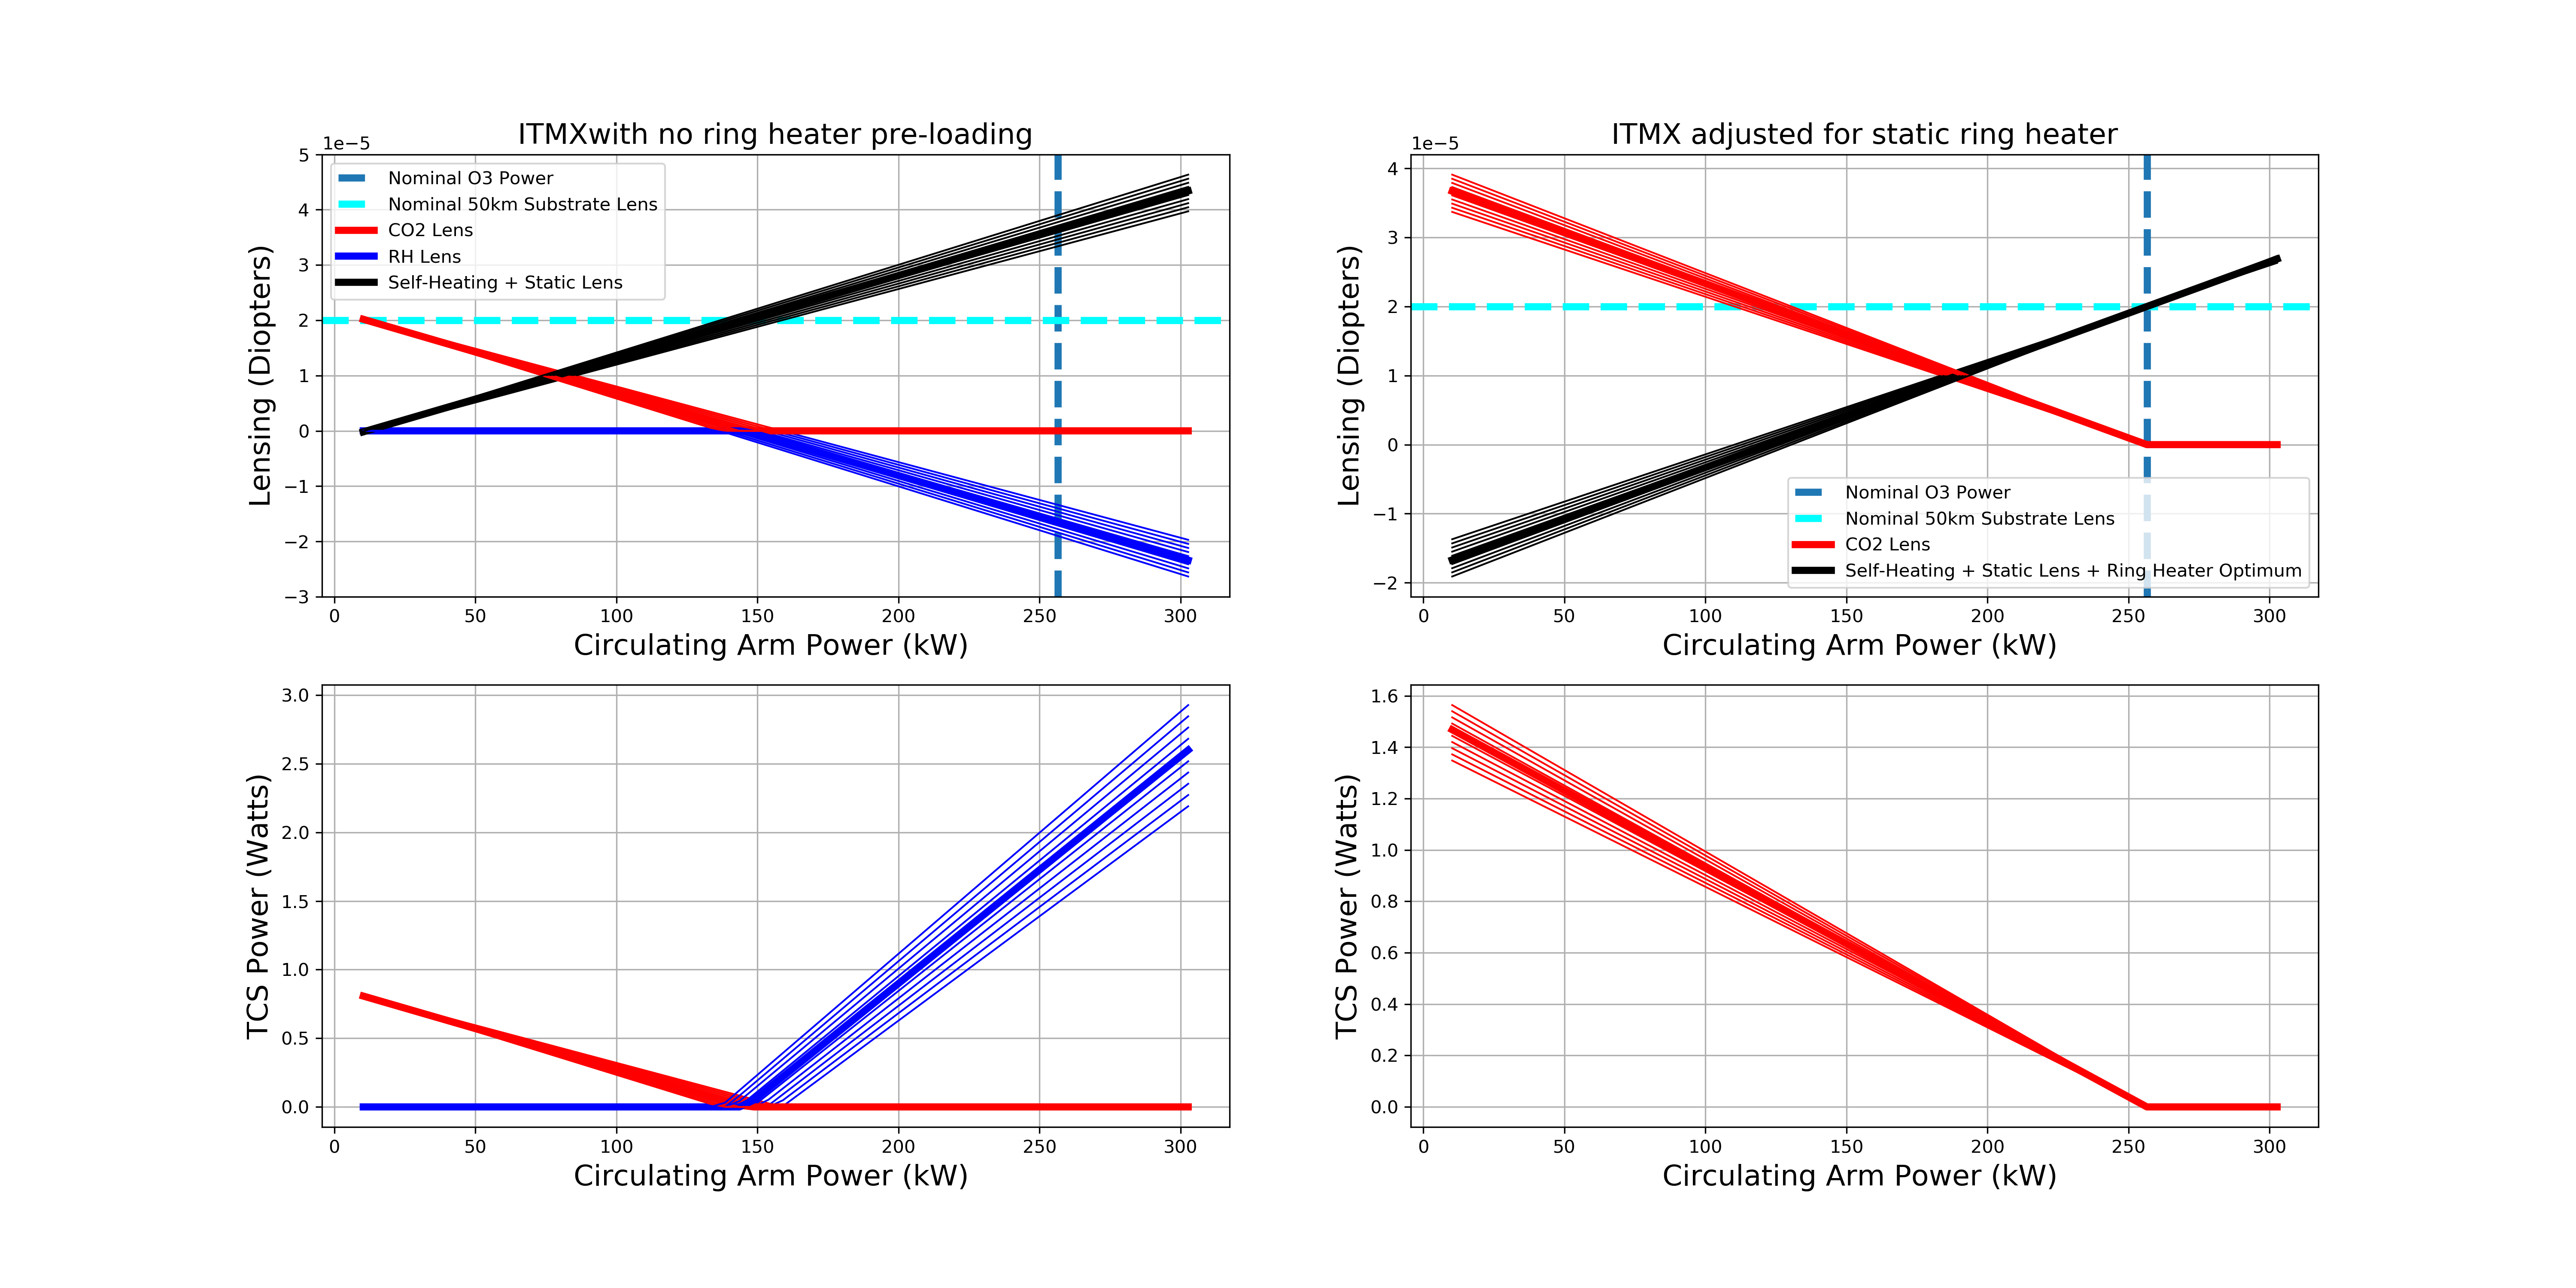
\includegraphics[width=\textwidth]{../Figures/ITMX_TCS_Settings.png}
			\label{fig:TCS_ITMX}
		\end{subfigure}
		\hfill
		\begin{subfigure}[b]{1.0\textwidth}
			\centering
			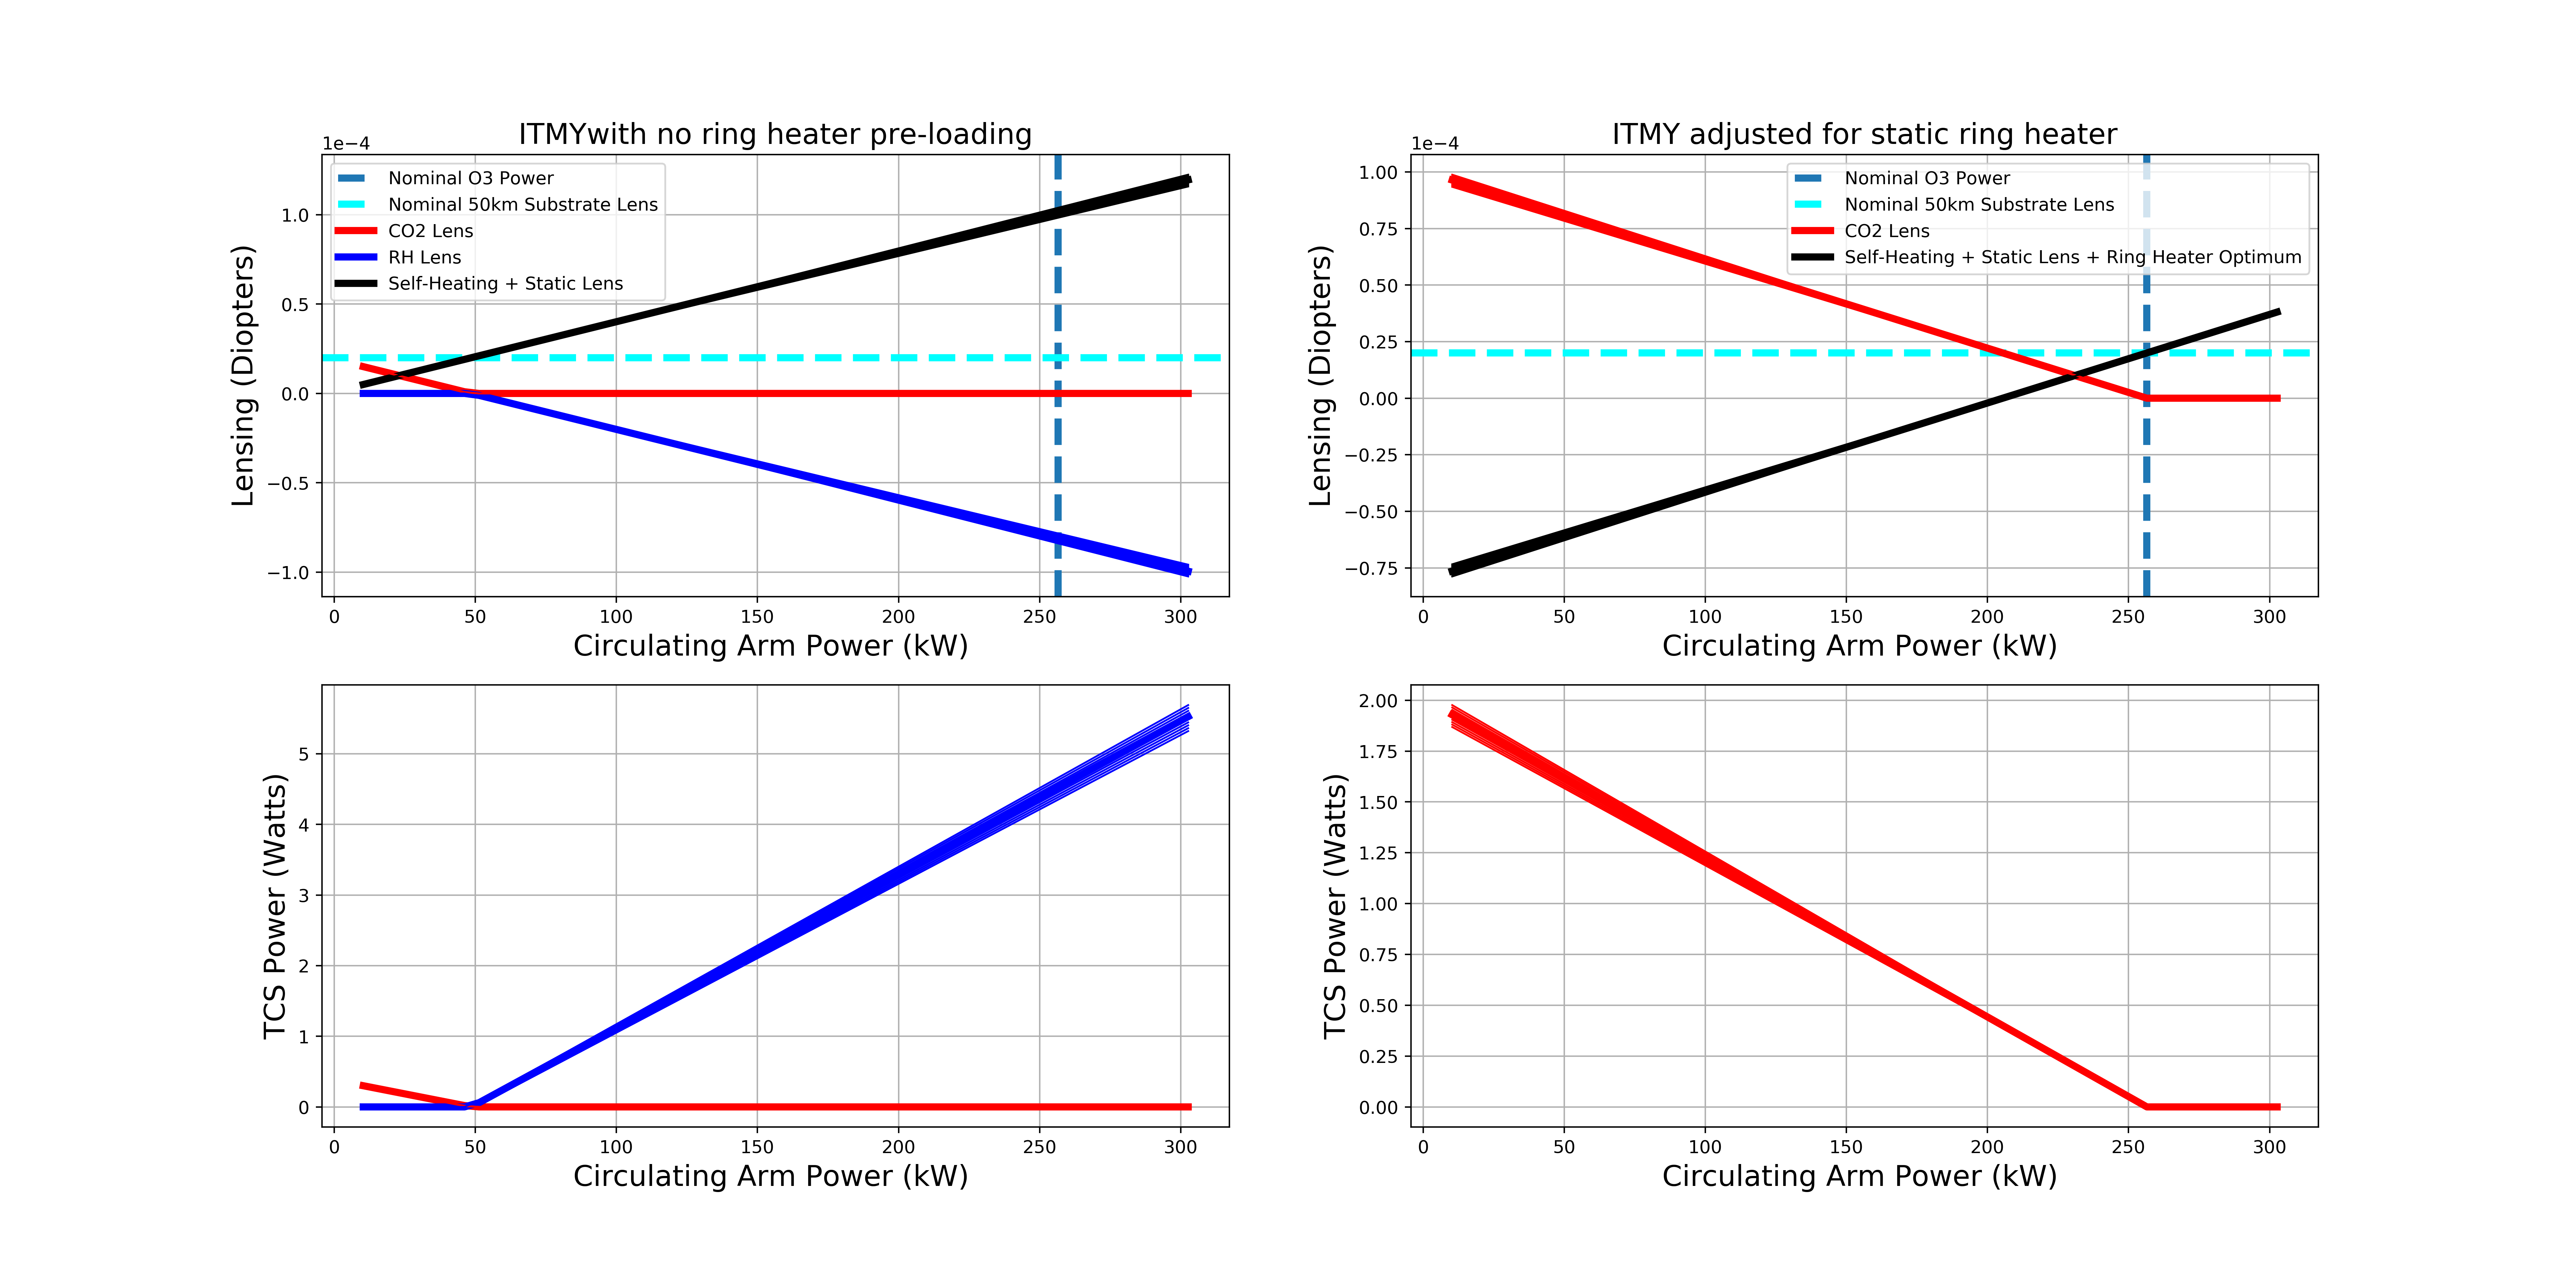
\includegraphics[width=\textwidth]{../Figures/ITMY_TCS_Settings.png}
			\label{fig:TCS_ITMY}
		\end{subfigure}
		\caption{The nominal circulating power denoted by the vertical blue line is a function of the input power, the recycling gain, and the arm cavity gain.  The nominal input power for O3 will be 50 Watts and the power recycling gain is around 45.  The arm cavity gain can be estimated by calibrating the transmitted power from each of the arms and is approximately 228.  The horizontal, dashed turquoise line represents the nominal substrate lens which the optics  }
		\label{fig:TCS_ITMs}
	\end{figure}
	
	\begin{figure}[ht]
		\centering
		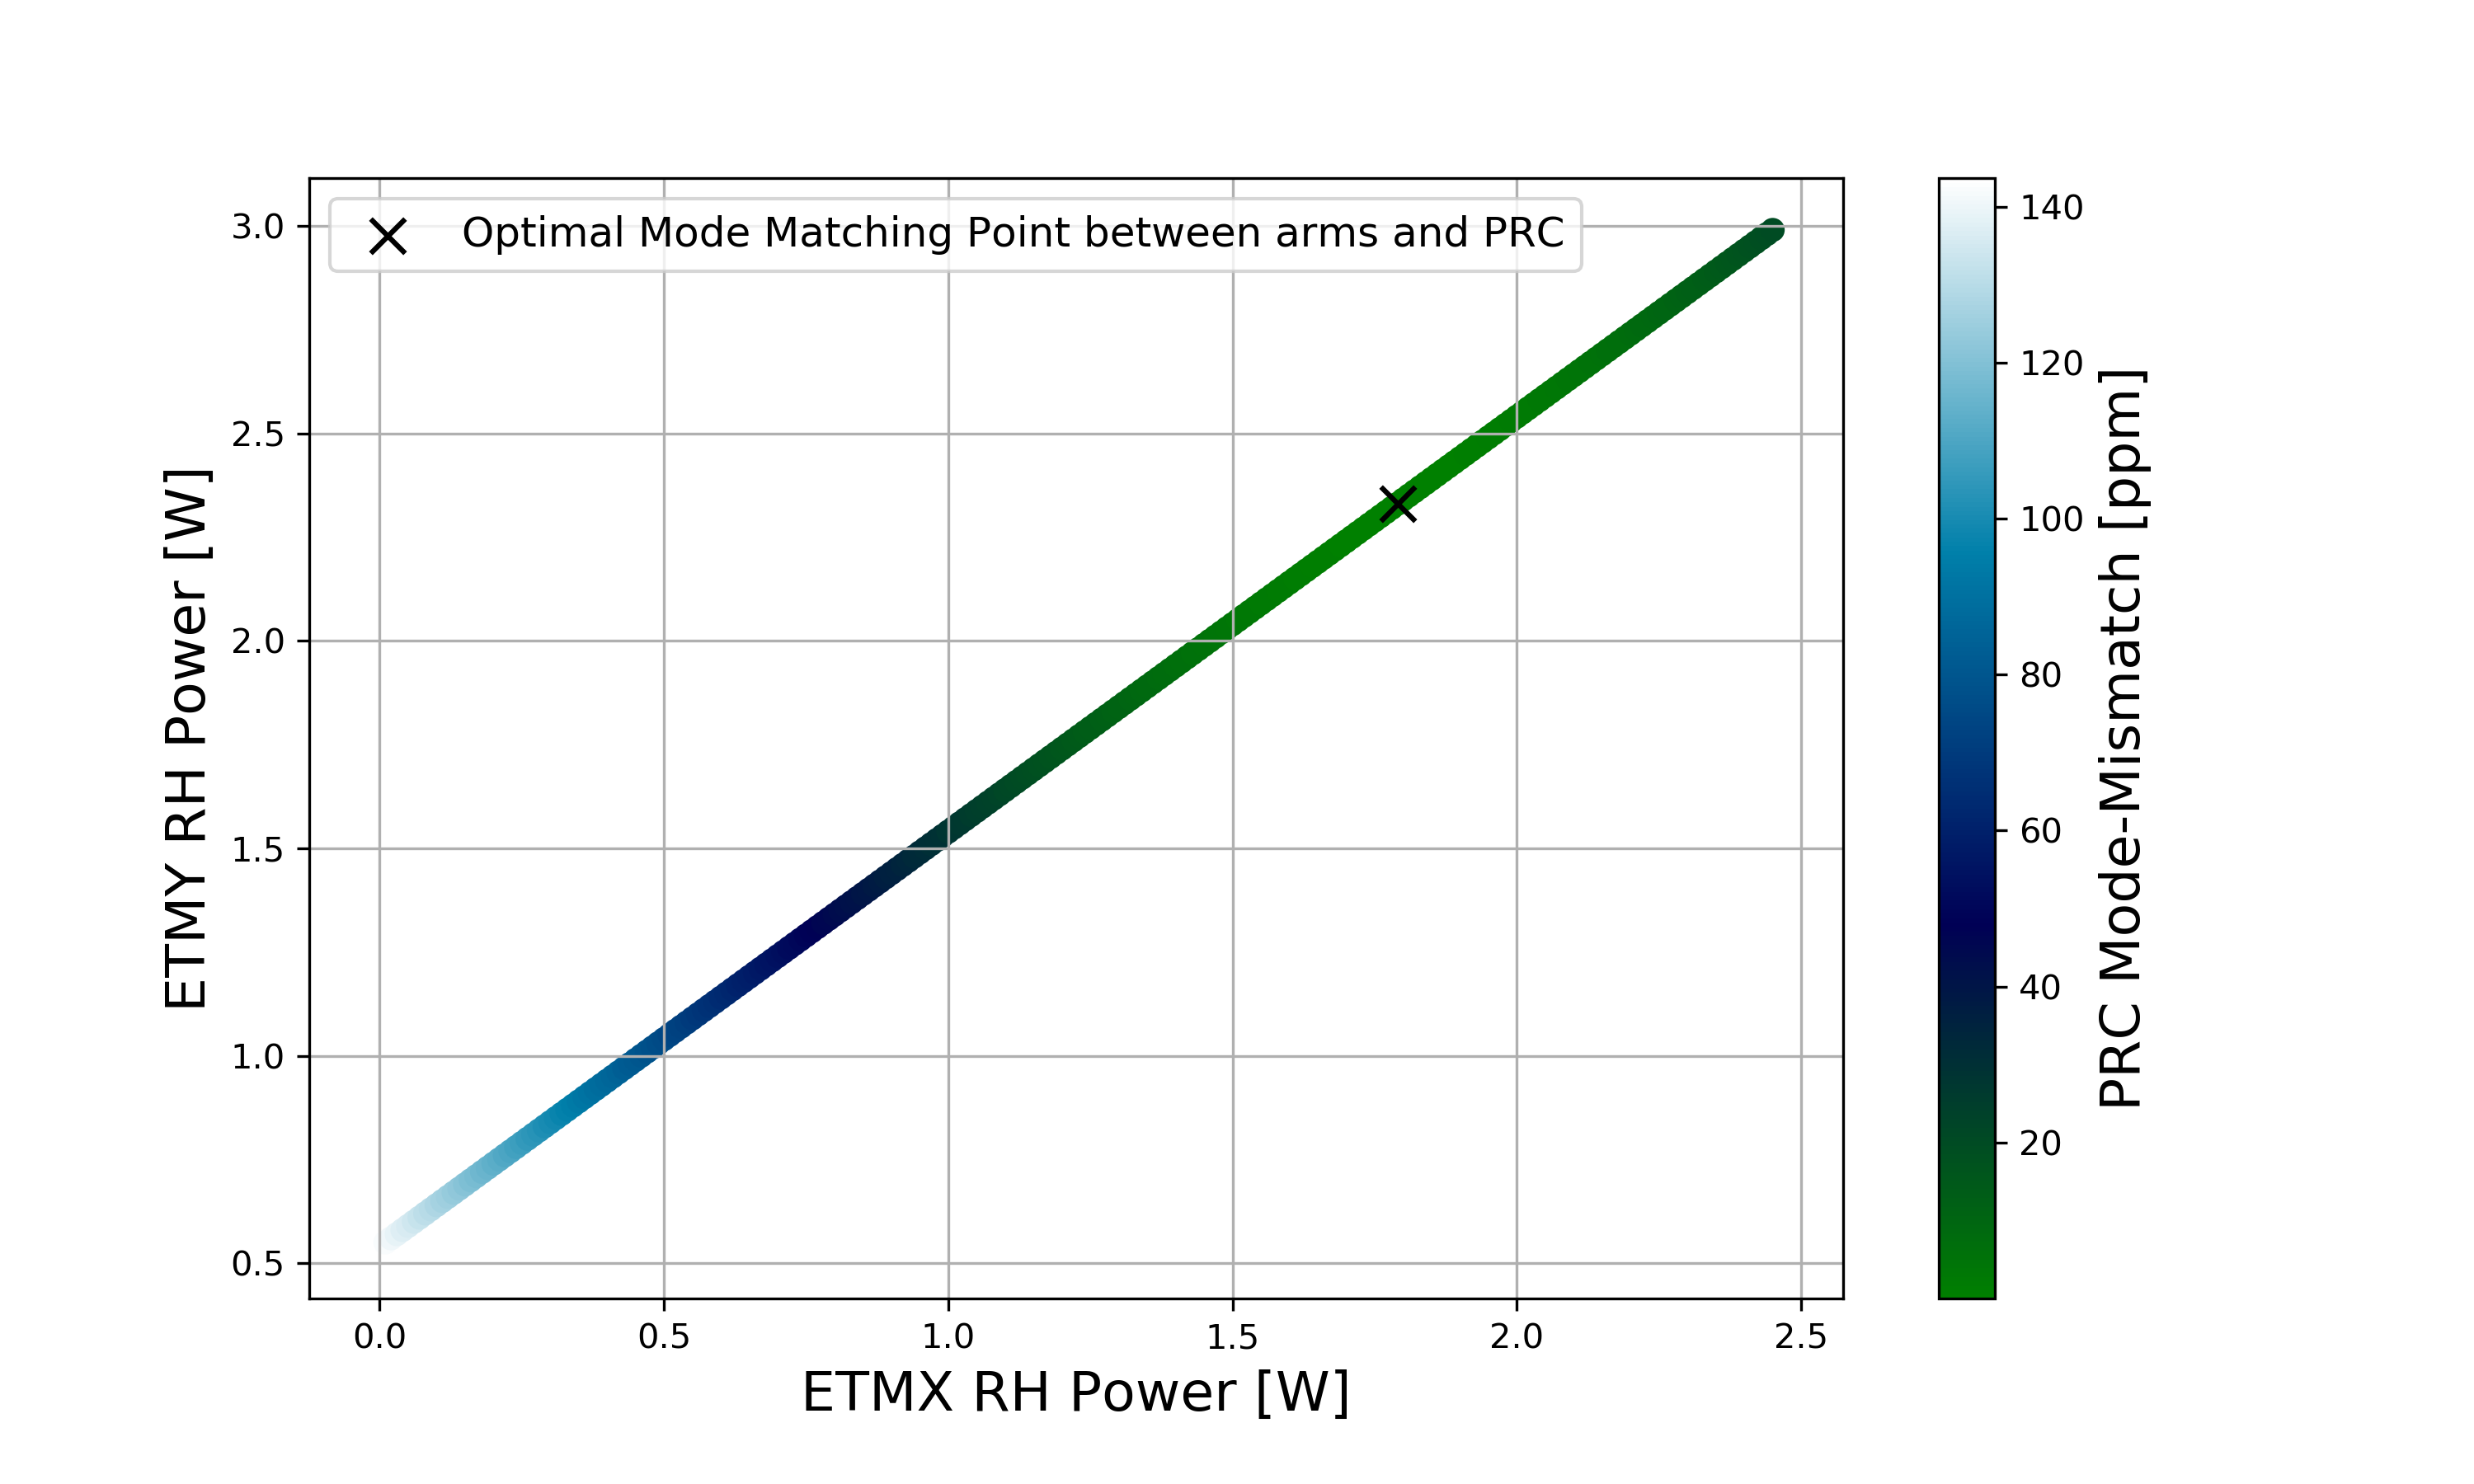
\includegraphics[width=1.0 \textwidth]{../Figures/ETM_TCS_Settings.png}
		\caption{Determining the ring heater and CO2 settings still leaves the end test mass ring heaters to be set.  The goal is to maintain the mode matching between the arms while simultaneously searching for the optimal overlap with the power recycling cavity. The linear portion of the graph shows a combination of common and differential adjustment of each ring heater that keeps the mode matching between the arms at less than 1 ppb, }
		\label{fig:TCS_ETM}
	\end{figure}
